\chapter{Abstract Stack Machine}

The notion of \emph{abstract machine} is a convenient concept in the field of programming languages, compliers and tools.
As the name suggests, abstract machine is a hypothetical computational device which fills the gap between a high-level language
and an actual hardware. It, therefore, introduces an additional intermediate abstraction level which facilitates the
decomposition of many compiler implementation and program analysis tasks. This decomposition makes it possible to separate
certain implementation subtasks, solve them and assess the correctness of solutions independently.

An important question is how an abstract machine can be specified and built. Do we need a blueprint, what appliances and equipment
should we use for its manufacturing? Fortunately, it turns out that we already have all what we need in our toolbox. For us an
abstract machine is just a language, and to specify an abstract machine we need to specify the syntax and semantics of
this language. Implementing an abstract machine amounts to implementing its interpreter. In this section we
give the syntax and semantics of a \lama-specific abstract stack machine, describe the compiler from straight-line
programs language into this abstract machine and prove its correctness. But, first, we briefly survey the variety of existing
flavours of abstract machines and discuss the motivation for the basic features of that we chose.

\section{The Variety of Abstract Machines}

Abstract machines share a lot of common features with actual hardware. They are programmable devices, and their
programs consist of instructions each of which is capable of performing a rather simple operation. On the other hand,
abstract machines often provide a direct way of representing and using \emph{meta-information} specific to a certain
lanaguage or a group of languages this abstract machine is devised to support. This may include types, object structures, etc.
For example, JVM directly supports such construct as virtual method call, which for a real hardware has to be
implemented using the knowledge of actual virtual methods table layout, etc. 



\begin{figure}[t]
  \centering

  \begin{subfigure}[t]{\textwidth}
   \centering
    $x*y+3$
    \caption{Expression}
    \label{expr}
  \end{subfigure}
  \vskip5mm
  \begin{subfigure}[t]{0.3\textwidth}
  \begin{verbatim}
      LD x
      LD y
      MUL
      CONST 3
      ADD
  \end{verbatim}  
  \caption{Stack Machine Code}
  \label{expr-stack}
  \end{subfigure}
  \begin{subfigure}[t]{0.3\textwidth}
  \begin{verbatim}
      MUL x, y, %1
      ADD %1, 3, %2


      
  \end{verbatim}  
  \caption{Three-address Code}
  \label{expr-3addr}
  \end{subfigure}
  \begin{subfigure}[t]{0.3\textwidth}
  \begin{verbatim}
      MOV y, %1
      MUL x, %1
      ADD 3, %1

      
  \end{verbatim}  
  \caption{Two-address Code}
  \label{expr-2addr}
  \end{subfigure}
  \caption{An Expression and Its Abstract Machine Code}
\end{figure}

There are different flavours of abstract machines. For now, as we are dealing with rather a simple language of
straight-line programs, only one essential feature is important: the representation of \emph{temporaries}.

In our language (and the majority of conventional programming languages) expressions can contain an arbitrary
number of operators. However, actual hardware (and the majority of abstract machines) cannot evaluate arbitrarily
large expressions ``in one step''. It evaluates them operator by operator, storing somewhere intermediate results, otherwise
called \emph{temporary values}. There are two major disciplines to work with temporaries:

\begin{itemize}
\item Using a \emph{stack}. With this discipline all temporary values are stored on a stack specifically disignated
  for this purpose. Thus, all operators take the operands from the stack and put the result back. This, in particular,
  means that the majority of instructions do not have explicit operands.
  
\item Using a potentially infinite number of named locations (often called \emph{pseudo-registers}). Under this approach
  the operands of each instruction (if any) are explicitly annotated. There are two commonly used special cases: \emph{three-address code},
  when an instruction can have up to three distinct operands (two for arguments and one for the result) and
  \emph{two-address code}, when an instruction can have no more than two operands, one of which serves simultaneously
  as an argument and as the result.
\end{itemize}

All these versions of abstract machines have their merits and shortcomings, and rather easier to switch to and from. Stack code is known
to be very compact (indeed, it does not require extra space to specify the operands for the majority of instructions); it is also a
little bit easier to generate. As the same time code with explicit operands is easier to analyize and transform, and faster to
interpret. It worth mentioning that the distinction stack vs. explicit operands by no means separates abstract machines from
real hardware: there some examples of the latter which implement stack architecture (the most notable, probably, is now late
Intel 8087 floating-point coprocessor).

In our case we favoured stack machine over others since the compilation to stack code posesses some nice invariants and
its correctness can be formally assessed easily. In addition the archiecture of \textsc{x86} is very close to two-address
code, so dealing with stack abstract machine allows us to consider a broader class of architectures.

\section{Syntax and Semantics}

The syntax of abstract stack machine language is shown below:

\[
\begin{array}{rcl}
  \mathscr{I} & = & \llang{BINOP$\;\otimes$}\\
              &   & \llang{CONST $\;\mathbb{N}$}\\
              &   & \llang{LD$\;\mathscr{X}$}\\
              &   & \llang{ST$\;\mathscr{X}$}\\
              &   & \llang{READ}\\
              &   & \llang{WRITE}\\[2mm]
  \mathscr{S} & = & \epsilon\\
              &   & \mathscr{I}\mathscr{S}
\end{array}
\]

We have here two syntactic categories~--- \emph{instructions} $\mathscr{I}$ and \emph{programs} $\mathscr{P}$.

There are six types of instructions, and only two types of programs~--- an empty program $\epsilon$ and a composite
program which consists of an instruction and a residual program. In essence the programs of stack machine
are just lists of instructions. Some of instructions have operands: for \llang{BINOP} an operand is a name of binary operator
from the source language, for \llang{CONST} it is a natural number, for \llang{LD} and \llang{ST}~--- the names of
variables. We can notice that the language of stack machine is very simple, much simpler than that for the straight-line programs. Yet it
possesses enough expressive power to perform the same calculations as an arbitrary straigh-line program! We assess this property
by implementing a compiler and proving its correctness.

Before giving a formal semantics for stack machine we first give an informal description of how it functions. The stack
machine operates in a similar environment as straight-line programs. It reads and writes numbers from/to a world, and it
posesses an internal state which binds (some) variables names to integer values. Beside that, stack machine has a
stack of integers at its discretion. In a nutshell, this stack contains temporary values which are nowhere to place
otherwise. The stack machine program executes instruction by instruction starting from the first instruction.
Each instruction modifies the configuration of the stack machine (state, stack, or world) and can either succeed or
fail (crash). The machine stops when there are no instructions left to execute; in this case the contents of
the output stream is taken as the result of stack program evaluation.

\setsubarrow{_{SM}}
\begin{figure}[t]
  \[
  \def\arraystretch{3}
  \arraycolsep=10pt
  \def\arraystretch{3}
  \begin{array}{cr} 
  \trans{c}{\epsilon}{c}&\ruleno{Stop$_{SM}$}\\
  \trule{\trans{\inbr{\sigma,\,(x\oplus y)s,\,\omega}}{p}{c^\prime}}{\trans{\inbr{\sigma,\,yxs,\,\omega}}{[\llang{BINOP $\;\otimes$}]p}{c^\prime}}&\ruleno{Binop$_{SM}$}\\
  \trule{\trans{\inbr{\sigma,\,zs,\,\omega}}{p}{c^\prime}}{\trans{\inbr{\sigma,\,s,\,\omega}}{[\llang{CONST $\;z$}]p}{c^\prime}}&\ruleno{Const$_{SM}$}\\
  \trule{\inbr{z,\,\omega^\prime}=\primi{read}{\;\omega},\,\trans{\inbr{\sigma,\,zs,\,\omega^\prime}}{p}{c^\prime}}{\trans{\inbr{\sigma,\,s,\,\omega}}{[\llang{READ}]\,p}{c^\prime}}&\ruleno{Read$_{SM}$}\\
  \trule{\trans{\inbr{\sigma,\,s,\,\primi{write}{\;z\;\omega}}}{p}{c^\prime}}{\trans{\inbr{\sigma,\,zs,\,\omega}}{[\llang{WRITE}]\,p}{c^\prime}}&\ruleno{Write$_{SM}$}\\
  \trule{\trans{\inbr{\sigma,\,(\sigma\;x)s,\,\omega}}{p}{c^\prime}}{\trans{\inbr{\sigma,\,s,\,\omega}}{[\llang{LD $\;x$}]p}{c^\prime}}&\ruleno{LD$_{SM}$}\\
  \trule{\trans{\inbr{\sigma\,[x\,\gets z],\,s,\,\omega}}{p}{c^\prime}}{\trans{\inbr{\sigma,\,zs,\,\omega}}{[\llang{ST $\;x$}]p}{c^\prime}}&\ruleno{ST$_{SM}$}
  \end{array}
  \]
  \caption{Big-step operational semantics for stack machine}
  \label{sm-bigstep}
\end{figure}

We describe this behavior, again, using a big-step operational semantics. First, we define the extended configuration $\mathscr{C}_{SM}$
for stack machine as

\[
\mathscr{C}_{SM}=St\times\mathbb{Z}^*\times\mathscr{W}
\]

Each component of extended configuration~--- state, stack of integers, word~--- is familiar to us. Next we need
to specify the big-step transition relation \mbox{``$\transrel$''} for stack machines. The rules of the semantics
are given in Fig.~\ref{sm-bigstep}. In the rules we additionaly surrounded the head instruction of a program
by square brackets \lstinline|[...]| to visually separate it from the rest of the program.

The first rule, \rulename{Stop$_{SM}$}, is at the same time the single axiom in the semantics. It tells us that an empty
program does not change the configuration. This, in particular, happens when all instructions of a program were
already evaluated and there is nothing left to evaluate.

All other rules follow the same pattern: they describe the effect of the first instruction of the current program,
and then prescribe to evaluate the rest of the program using the same evluation relation.

Rule \rulename{Binop$_{SM}$} describes the case when the first instruction is a binary operator. To succeed, this instruction
requires atleast two integer values, $x$ and $y$, to reside on the stack. If so, it combines these values using binary
operator $\oplus$ and puts the result back on the stack. The correspondence between ``$\otimes$'' and ``$\oplus$'' is,
of course, the same as for the semantics of straght-line programs (see a table of the page~\pageref{times-plus-tab}).

Rule \rulename{Const$_{SM}$} corresponds to the case when the first instruction is \llang{CONST$\;z$}. This instruction
puts its operand $z$ on the stack.

The next two symmetrical rules, \rulename{Read$_{SM}$} and \rulename{Write$_{SM}$}, deal with instructions \llang{READ} and
\llang{WRITE} respectively. \llang{READ} reads a value from input stream and puts it on the stack; if the input stream is
empty the instruction fails. \llang{WRITE} takes a valus from the top of the stack and puts it in the output stream; this
instruction fails if the stack is empty.

Finally, two last rules, \rulename{LD$_{SM}$} and \rulename{ST$_{SM}$}, desribe the semantics of instructions \llang{LD} and
\llang{ST}. Both instructions have an operand, the name of a variable. \llang{LD$\;x$} puts the value of variable $x$, associated
in the current state $\sigma$, on the stack. It fails if $\sigma\;x$ is undefined. \llang{ST$\;x$} takes the top value from the
stack and updates the current state $\sigma$ to associate $x$ with this value. It fails if the stack is empty.

With the transition relation $\transrel$ defined we can specify the ``surface'' semantics for stack machine programs $\sembr{\bullet}^\ph_{SM}$:

\[
  \begin{array}{c}
    \sembr{\bullet}^\ph_{SM} : \mathscr{S}\to \mathbb{Z}^*\to \mathbb{Z}^*\\[2mm]
      \trule{\trans{\inbr{\Lambda,\,\epsilon,\,\inbr{i,\,\epsilon}}}{p}{\inbr{\sigma,\,s,\,\omega}}}
            {\sembr{p}^\ph_{SM}\;i=\primi{out}{\;\omega}}
  \end{array}
\]

In other words, we take an input $i$, create an initial configuration, consisting of an empty state $\Lambda$, empty stack $\epsilon$ and an
initial world $\inbr{i,\,\epsilon}$, then run the program and, if it eventually comes to an end with some final configuration $\inbr{\sigma,\,s,\,\omega}$, we take
output stream from this configuration's world as the result of the evaluation.

As always, we can identify the following important properties of the semantics:

\begin{itemize}
\item \emph{Determinism:} for each program and each configuration there is at most one rule that can be applied; thus, if (for arbitrary $i$ and $p$)
  $\sembr{p}^\ph_{SM}\;i=o$ and   $\sembr{p}^\ph_{SM}\;i=o^\prime$ then $o=o^\prime$;
\item \emph{Compositionality}: the premise of each rule deals with programs one instruction shorter, than the conclusion. This, again, means that
  the principle of structural induction can be applied for proving the properties of the semantics.
\end{itemize}

It is also worth discussing the ``shape'' of derivation which the rules of the semantics generate. As we can see, each rule (except for the axiom) has
exactly one premise, and the final configuration of the primise is at the same time the final configuration of the conclusion. This means that
the derivations in this semantics have the form of a ``tower''; the top of the tower corresponds to the application of the single axiom, which
transfers its initial configuration to final one unchanged, and after that this final configuration is propagated down the tower in the right-hand side
configurations of all involved rules. The effects of individual instructions can be traced in the bottom-up manner in the left-hand side configurations of the
rules comprising the tower. To illustrate this structure, consider the following stack machine program:

\begin{verbatim}
   READ
   READ
   BINOP +
   WRITE
\end{verbatim}

The derivation ``tower'' which corresponds to the evaluation of this program for the input $\inbr{2,\,3}$ is shown in Fig.~\ref{derivation-tower}. As always,
we omit program for space considerations; the solid arrows connect the ``floors'' of the tower while dashed ones show the configurations' data flow.

\begin{figure}[h]
  \centering
  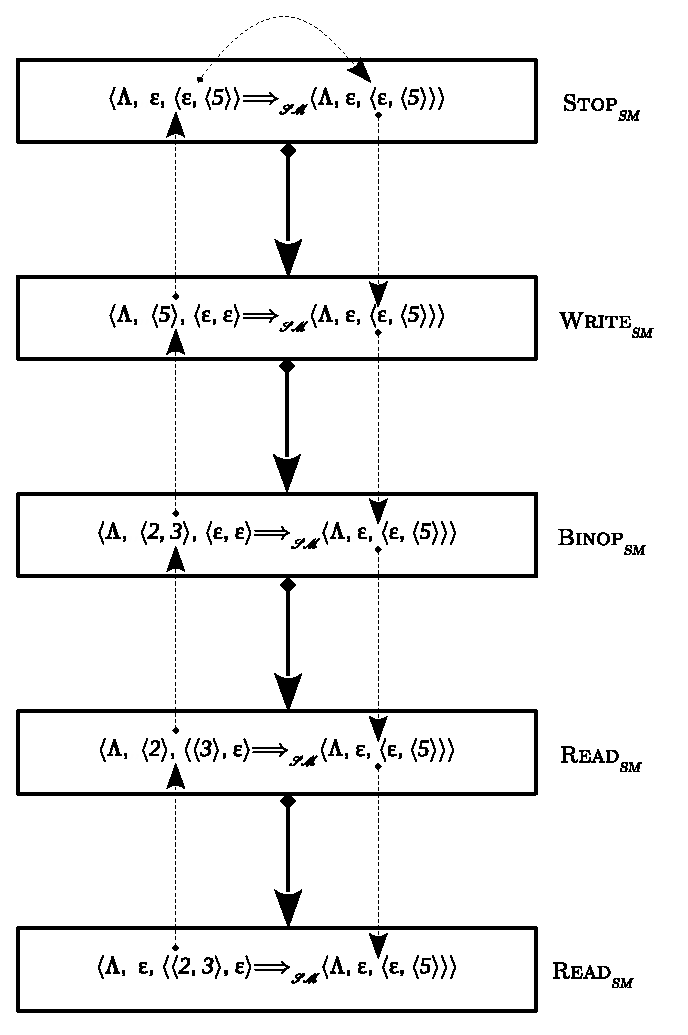
\includegraphics[scale=0.8]{images/05-01.eps}
  \caption{Derivation ``tower'' example}
  \label{derivation-tower}
\end{figure}

\subsection{Composition property}

In order to assess the correctness of compilation we need to formally establish a rather expected property of stack machine programs. Let assume
that we have a program $p$ and there are two configurations $c$ and $c^\prime$ such that

\[
\trans{c}{p}{c^\prime}
\]

In other words, $p$, being evaluated for the configuration $c$, completes succesfully with the final configuration $c^\prime$. As the instructions 
of $p$, according to the semantics, are evaluated succesively one after another this should mean that each \emph{subprogram} (a continuous sublist
of instructions) of $p$ completes succesfully for some configurations, derived from $c$.

In order to reify this expectation into a formal claim we need to define a concatenation of programs ``$\dplus$'':

\[
\begin{array}{rclcl}
\epsilon & \dplus & p       & = & p\\
\iota\,p & \dplus & p^\prime & = & \iota\,(p \dplus p^\prime)
\end{array}
\]

We need this operation since there is no other way to ``join'' programs together: we cannot just take program $q$ and program $t$ and consider $pq$ as
a program since there is no such syntactic form. Operation ``$\dplus$'' is defined inductively on the first operand; it is, in essence, a list
concatenation function.
\FloatBarrier

Now we can formulate the following lemma.

\begin{lemma}[Composition property]
  Let $p$, $q$, and $t$ be stack machine programs such that $p=q\dplus t$. Then if for some configurations $c$ and $c^\prime$

  \[
  \trans{c}{p}{c^\prime}
  \]

  then there exists a configuration $c^{\prime\prime}$ such that

  \[
  \trans{c}{q}{c^{\prime\prime}}\mbox{ and  }\trans{c^{\prime\prime}}{t}{c^\prime}
  \]
\end{lemma}
\begin{proof}
  The proof, of course, goes by induction on the structure of $q$.

  The base case is $q=\epsilon$. Then $p=\epsilon\dplus t=t$ and the lemma follows vacuously by taking $c^{\prime\prime}=c$.

  Let $q=\iota\,q^\prime$. Then $p=q\dplus t=\iota\,(q^\prime\dplus t)$. Obviously, there exists a configuration $\widetilde{c}$ such that

  \[
  \trans{c}{\iota\,\epsilon}{\widetilde{c}}
  \]

  since there is no way to complete the evaluation of $p$ with the final configuration $c^\prime$ if its first instruction fails. So
  when we evaluate $p$ in configuration $c$ we have to evaluate $q^\prime\dplus t$ in configuration $\widetilde{c}$. But we
  can apply induction hypothesis here since $q^\prime$ is a subprogram of $q$. Thus, there exists $c^{\prime\prime}$ such that

  \[
  \trans{\widetilde{c}}{q^\prime}{c^{\prime\prime}}\mbox{ and  }\trans{c^{\prime\prime}}{t}{c^\prime}
  \]

  But from

  \[
  \trans{c}{\iota\,\epsilon}{\widetilde{c}}
  \]

  and

  \[
  \trans{\widetilde{c}}{q^\prime}{c^{\prime\prime}}
  \]

  and the determinism of the semantics it follows

  \[
  \trans{c}{\iota\,q^\prime=q}{c^{\prime\prime}}
  \]

  which completes the proof.
\end{proof}

The conversion of this property is also true: let $p$ and $q$ be such programs that

\[
\trans{c}{p}{c^\prime}\mbox{ and }\trans{c^\prime}{q}{c^{\prime\prime}}
\]

for some configurations $c$, $c^\prime$ and $c^{\prime\prime}$. Then

\[
\trans{c}{p\dplus q}{c^{\prime\prime}}
\]

The proof is similar and left to the reader.

\section{Stack Machine Interpreter}

Our next task is implementing the interpreter for stack machine. Given the simplicity of the language one may wonder if
this subject deserves a separate section.

It definitely would not if we, indeed, were going to present only the same kind of interpreter (actually called
\emph{simple recursive interpreter}) as for the straight-line programs language. However, in the case of
abstract machines the assortment of approaches to interpreter implementation is much broader. Indeed, unlike source-level interpreters,
which main feature is to follow the semantics as close as possible, abstract machine interpreters often play the role of
a real runtime environment. Thus, the performance issue comes up.

We consider here three types of interpreters: the simple recursive one, iterative non-recursive, and \emph{threaded code} interpreter. It is worth
mentioning that, as long as we implement these kinds of interpreters in \lama, their performance will remain roughly the same. However,
``the real'' abstract machine interpreters as a rule are implemented in a lower level than \lama languages~--- \textsc{C} or, perhaps,
assembler, and in those languages the techniques we discuss indeed deliver essential speedup.

Our first interpreter (Fig.~\ref{simple-recursive}) literally encodes the operational semantics. Stack machine program (\lstinline|insns|) is
represented as a list of instructions, and each instruction is directly represented as an S-expression. The big-step transition relation is
encoded using nested function \lstinline|eval| which takes a configuration and a program, branches on the first instruction 
(if any), calculates the next configuration and recursively calls itself with the new configuration and the remaining
part of the program. The branching corresponds to the choice of the semantics' rule, recursive call~--- to the calculation in rule's
primise, and the case of empty list~--- to the application of the axiom. It is easy to see that the configuration of recursive calls
repeats the shape of derivation ``tower'': unless the program is non-empty the interpreter keeps calling itself with updated
configuration, and once the program ends the final configuration is propagated as the return value of resursive calls. The
function \lstinline|evalOp| is exactly the same as in Fig.~\ref{binary-int}, which is unsurprising since it is exactly the same
in the semantics as well. The ``surface'' semantics $\sembr{\bullet}_{SM}$ is implemented by the function \lstinline|evalSM|, which
takes an input stream, a program, makes initial configuration, runs the machine and returns the output stream of the final
configuration (if any).

\begin{figure}
  \begin{lstlisting}
fun evalSM (input, insns) {
  fun eval (c@[st, s, w], insns) {
    case insns of
      {} -> c
    | i : insns ->
        eval (
          case i of
            READ       -> let [n, w] = readWorld (w) in
                           [n : st, s, w]
          | WRITE      -> let n : st = st in
                           [st, s, writeWorld (n, w)]    
          | BINOP (op) -> let y : x : st = st in
                           [evalOp (op) (x, y) : st, s, w] 
          | CONST (n)  -> [n : st, s, w]
          | LD    (x)  -> [s (x) : st, s, w]
          | ST    (x)  -> let n : st = st in
                           [st, s <- [x, n], w] 
          esac,
          insns
        )
    esac
  }
     
  eval ([{}, emptyState, createWorld (input)], insns)[2].getOutput
}
  \end{lstlisting}
  \caption{Simple recursive interpreter}
  \label{simple-recursive}
\end{figure}

The interpeter of this kind is an ideal tool to provide a literal encoding for the semantics. However, from the performance standpoint
it lacks a lot. First of all, it is easy to see that the depth of recursive calls is equal to the length of the program being interpreted.
This means that for long programs the interpreter most likely will crush due to the call stack overflow (unless \lama compiler implements a special
transformation called \emph{tail call elimination}). Then, we represent programs as lists, which is completely ok if the objective is
to follow the specification literally. However, it is rather obvious that this representation is excessive: as programs do
not change in the course of interpretation we pay extra space taken by lists for nothing. In addition lists are not random-access
structures~--- we can not get their arbitrary elements without extra efforts. In our case when programs are executed strictly
successively this does not matter as we only take the tail of a list (in \emph{constant} time) each time we switch to the next
instruction. However, for more advanced languages with control flow this will no longer be the case, and the slow access to an
arbitrary instruction can become an issue. Similarly, we represent states as functions in strong accordance with the semantics; however
is is obvious that from performance standpoint this representation is not the best choice~--- there is only a finite number of
variables in each program, and this number does not change.

Thus, our next version is a \emph{simple iterative} iterpreter. We make the following changes to the program and configuration
representations:

\begin{itemize}
\item we represent programs as \emph{arrays} of instructions rather then lists;
\item we represent variables by numbers, not names;
\item we represent states as arrays of numbers, indexed by variables.
\end{itemize}

These changes require a conversion of initial program and configuration representations to the new one~--- we need, for example, enumerate
all varables in given program, etc. The implementation of this simple conversion is left to the reader. The iterative interpreter
is shown in Fig.~\ref{simple-iterative}. The interpreter takes an input, a program as array of instructions, and a number of
variables in the program. As the interpreter simply iterates over the instructions' array (using integer variable \lstinline|ip|, ``instruction pointer''),
we no longer need nested recursive function. We keep stack, world, and state as mutable data structures and provide helper functions
\lstinline|push| and \lstinline|pop| to encapsulate conventional operations for the stack. The state is represented as an array of
integers, and we use regular array access constructs of \lama to operate on the state. Otherwise, the implementation resembles that for
simple recursive case. We still represent the instructions as S-expressions, although now the arguments of instructions \texttt{LD} and \texttt{ST}
are integers, not strings. If we were implementing the interpreter in a lower level language like \textsc{C} we, probably, would use
another enoding for the instructions using integer numbers/bit-field structures, which would improved the performance even more, but as the
demonstration of the idea this version is sufficient.

There is, however, one interesting and important observation which we have to make: as we switched from state-as-functions to state-as-arrays
representation we lost the ability to detect the use of non-initialized variables! Thus, strictly speaking we \emph{do not}
have a fully correct interpreter anymore, but only a partially correct. For example, the semantics of the program

\begin{lstlisting}
   LD x
   WRITE
\end{lstlisting}

is undefined function, but simple iterative interpreter would write 0 for each input, this implementing a \emph{different} semantics. We could, of course,
resurrect this lost feature by representing states not by arrays of integers, but by arrays of, say, options; this choice, however, would hamper the
performance, questioning the very idea of switching the representation for states. This is rather a typical scenario in the field: in order to
make the implementation more efficient we sometimes have to deviate from the puristic interpretation of the semantics by allowing programs to ignore
some (but not all!) ``pathological'' situations. We can not, however, take these decisions arbitrarily; partial correctness sets the boundary
which we should not cross.


\begin{figure}
  \begin{lstlisting}[mathescape=true]
var st;

fun push (n) {
  st := n :: st      
}

fun pop () {
  let x :: st' = st in
  st := st';
  x
}

fun evalSMiterative (input, [insns, numVars]) {
  var ip, w = createWorld (input);  
  val s = initArray (numVars, fun (_) {0});
  
  st := {};

  for ip := 0, ip<insn.length, ip := ip+1 do
    case insn [ip] of
      READ       -> let [n, w'] = readWorld (w) in                    
                     push (n);
                     w := w'
    | WRITE      -> w := writeWorld (pop (), w)
    | BINOP (op) -> let y = pop () in
                     let x = pop () in
                     push (evalOp (op) (x, y))
    | CONST (n)  -> push (n)
    | LD    (x)  -> push (s [x])
    | ST    (x)  -> s[x] := pop ()
    esac
  done;

  getOutput (w)
}
  \end{lstlisting}
  \caption{Simple iterative interpreter}
  \label{simple-iterative}
\end{figure}

Our final kind of interpreter is \emph{direct threaded code} interpreter. The idea behind this approach is quite simple: we represent each
instruction as a function which, being called, performes the same actions as this instuction. Again, as long as we write in \lama this
representation probably would not deliver us any performance gain; however this technique is a yet another good pattern when using
lower-level languages. The benefit of threaded code is that we do not need pattern matching anymore: as each instruction
``knows'' what to do itself in the main loop of the interpreter we just need to call each function from program array. The
implementation of the interpreter is shown in Fig.~\ref{threaded-interpreter}. Similarly to the previous case we
represent the elements of configurations as mutable variables, and for each instruction we provide a function which encodes its semantics.
If the instruction in question does not have arguments we can write such a function once and for all; otherwise we need to capture the arguments
in the enclosed nested function definition. The main function of the interpreter, again, takes an input, a program in the form of array of
functions, and a number of variables. It initializes the configuration and runs throught the program, calling each instruction function.

\begin{figure}
  \begin{lstlisting}[mathescape=true]
var st, s, w;
    
fun binop (op) {
  fun () {
    let y = pop () in
    let x = pop () in
    push (evalOp (op) (x, y))
  }
}

fun ld (x) {
  fun () {
    push (s [x])
  }
}

fun st (x) {
  fun () {
    s [x] := pop ()
  }
}

fun const (n) {
  fun () {
    push (n)
  }
}

fun read () {
  let [n, w'] = readWorld (w) in
  s [x] := n;
  w      w'
}

fun write () {
  w := writeWorld (pop (), w)
}

fun evalSMthreaded (input, [insns, numVars]) {
  var ip;
  
  s  := initArray (numVars, fun (_) {0});
  st := {};
  w  := createWorld (input);
  
  for ip := 0, ip<insn.length, ip := ip+1 do
    insn [ip] ()
  done;

  getOutput (w)
}
  \end{lstlisting}
  \caption{Threaded code interpreter}
  \label{threaded-interpreter}
\end{figure}

\section{Stack Machine Compiler}

In this section we describe a compiler from straigh-line programs language to the abstract stack machine and prove its correctness.
The first question is what ``describe'' means. Recall, we already dealt with two understandings of a compiler:

\begin{itemize}
\item as a total syntactic transformation from one programming language to another;
\item as a \emph{program} which implements such a transformation.
\end{itemize}

Does it not resemble \emph{semantics} and \emph{reference interpreter}? Let us want to implement a compiler

\[
comp : L_1\to L_2
\]

from $L_1$ to $L_2$. Obviously, we can consider it as a semantics of $L_1$ with semantic domain $L_2$. This might look contrived or
exotic, but, in fact, in the earlier days there existed a (rather extreme) standpoint that the semantics of a language is
determined by its compiler. If compiler is a semantics, then its implementation as a program is this semantics' interpreter! While
we may argue if this point of view is desirable from a methodological perspective, we can atleast agree that even if not we can still
use precisely the same tools we used to specify the semantics to specify a compiler.

In a nutshell, we have to define a transformation

\[
\sembr{\bullet}^\ph_{comp}:\mathscr{S}\to\mathscr{P}
\]

such that for arbitrary program $p\in\mathscr{S}$

\[
\sembr{\sembr{p}^\ph_{comp}}^\ph_{SM}=\sembr{p}^\ph_\mathscr{S}\eqno{(\clubsuit)}
\]

As our source language consists of two syntactic categories, we additionally need to provide a compiler for expressions $\sembr{\bullet}^\mathscr{E}_{comp}$.
In fact, due to the simplicity of both source and target languages, the compiler is quite simple as well. The specification of compiler is shown in
Fig.~\ref{expr-comp} and Fig.~\ref{stmt-comp}. As we can see we used an already familiar denotational style when the result of compilation is
directly specified. All expected properties~--- compositionality and determinism,~--- are provided trivially, so we atlest can immediately
conclude that we specified a total function. But why this function indeed provides a correct compilation? We consider this question in the next
section.

\begin{figure}
\[
\begin{array}{rcl}
  \sembr{x}^{\mathscr E}_{comp}&=&\llang{[LD $\;x$]}\\
  \sembr{n}^{\mathscr E}_{comp}&=&\llang{[CONST $\;n$]}\\
  \sembr{A\otimes B}^{\mathscr E}_{comp}&=&\sembr{A}^{\mathscr E}_{comp}\dplus\sembr{B}^{\mathscr E}_{comp}\dplus[\llang{BINOP $\;\otimes$}]
\end{array}
\]
\caption{Stack machine compiler for expressions}
\label{expr-comp}
\end{figure}

\begin{figure}
\[
\begin{array}{rcl}
  \sembr{\llang{$x$ := $e$}}^\ph_{comp}&=&\sembr{e}^{\mathscr E}_{comp}\dplus\llang{[ST $\;x$]}\\
  \sembr{\llang{read ($x$)}}^\ph_{comp}&=&\llang{[READ][ST $\;x$]}\\
  \sembr{\llang{write ($e$)}}^\ph_{comp}&=&\sembr{e}^{\mathscr E}_{comp}\dplus\llang{[WRITE]}\\
  \sembr{\llang{$S_1$;$\;S_2$}}^\ph_{comp}&=&\sembr{S_1}^\ph_{comp}\dplus\sembr{S_2}^\ph_{comp}
\end{array}
\]
\caption{Stack machine compiler for statements}
\label{stmt-comp}
\end{figure}

\subsection{Correctness of the Compiler}

We are going to prove the correctness of the compiler, the property formally expressed by the equation $(\clubsuit)$. Both $\sembr{\bullet}^\ph_{SM}$ and $\sembr{\bullet}^\ph_\mathscr{S}$ are
defined in terms of corresponding transition relations, so we, apparently, need some statements concerning those relations as well. In addition we need to relate somehow
the transition relation ``$\transrel$'' for stack machines and denotational semantics for expressions $\sembr{\bullet}^\ph_\mathscr{E}$. Fortunately, the overall task turns out
to be not so demanding as it might look at the first glance if an appropriate set of lemmas is formulated.

\begin{lemma}{Correcntess of expression compiler.}
  Let $e\in\mathscr{E}$ be an expression, $\sigma\in St$~--- some state, $s\in\mathbb Z^*$~--- stack, $\omega\in\mathscr{W}$~--- some world, and $z\in\mathbb Z$~--- some number. Then

  \[
  \trans{\inbr{\sigma,\,s,\,\omega}}{\sembr{e}^\mathscr{E}_{comp}}{\inbr{\sigma,\,zs,\,\omega}}\Longleftrightarrow\sembr{e}^\ph_\mathscr{E}\,\sigma=z
  \]  
\end{lemma}
\begin{proof}
  Both directions can be proven by structural induction on $e$. We do this only in the reverse direction (``$\Leftarrow$'') and leave the other to the reader.
  \begin{itemize}
  \item[Base case.] Let $e=x\in\mathscr{X}$ By the definitions of $\sembr{\bullet}^\mathscr{E}_{comp}$ and $\sembr{\bullet}^\ph_\mathscr{E}$ we have:

    \[
    \begin{array}{rcl}
      \sembr{x}^\mathscr{E}_{comp}&=&\llang{[LD$\,x$]}\\
      \sembr{x}^\ph_\mathscr{E}\,\sigma&=&\sigma\,(x)
    \end{array}
    \]

    By the condition of the lemma $\sigma\,(x)=z$. Finally, by the definition of ``$\transrel$'' we have

    \[
    \trans{\inbr{\sigma,\,s,\,\omega}}{[\llang{LD$\,x$}]}{\inbr{\sigma,\,zs,\,\omega}}
    \]

    The second case ($e=n\in\mathbb N$) is established similarly.

  \item[Induction step.] Let $e=l\otimes r$ and let the lemma holds for $l$ and $r$. Again, by the definitions of $\sembr{\bullet}^\mathscr{E}_{comp}$ and $\sembr{\bullet}^\ph_\mathscr{E}$ we have:
    
    \[
    \begin{array}{rcl}
      \sembr{l\otimes r}^\mathscr{E}_{comp}&=&\sembr{l}^\mathscr{E}_{comp}\dplus\sembr{r}^\mathscr{E}_{comp}\dplus\llang{[BINOP$\,\otimes$]}\\[2mm]
      \sembr{l\otimes r}^\ph_\mathscr{E}\,\sigma&=&\sembr{l}^\ph_\mathscr{E}\,\sigma\oplus\sembr{r}^\ph_\mathscr{E}\,\sigma
    \end{array}
    \]

    From the condition of the lemma we know that $\sembr{l}^\ph_\mathscr{E}\,\sigma=x$ and $\sembr{r}^\ph_\mathscr{E}\,\sigma=y$ for some $x$ and $y$, and that

    \[
    \begin{array}{c}
      \trans{\inbr{\sigma,\,s,\,\omega}}{\sembr{l}^\mathscr{E}_{comp}}{\inbr{\sigma,\,xs,\,\omega}}\\[2mm]
      \trans{\inbr{\sigma,\,xs,\,\omega}}{\sembr{r}^\mathscr{E}_{comp}}{\inbr{\sigma,\,yxs,\,\omega}}
    \end{array}      
    \]

    Applying the composition property twice we get

    \[
    \begin{array}{c}
      \trans{\inbr{\sigma,\,s,\,\omega}}{\sembr{l}^\mathscr{E}_{comp}\dplus\sembr{r}^\mathscr{E}_{comp}}{\inbr{\sigma,\,yxs,\,\omega}}\\[2mm]
      \trans{\inbr{\sigma,\,s,\,\omega}}{\sembr{l}^\mathscr{E}_{comp}\dplus\sembr{r}^\mathscr{E}_{comp}\dplus\llang{BINOP$\,\oplus$}}{\inbr{\sigma,\,(x\otimes y)s,\,\omega}}
    \end{array}
    \]

    But $x\oplus y=\sembr{l\otimes r}\,\sigma$ which exists by the condition of the lemma.    
  \end{itemize}
\end{proof}

This lemma ensures the correctness of compliation for expressions: a compiled from an expression stack machine program being executed for some configuration
succesfully finishes and leaves on the stack the value of this expression in this configuration's state if and only if the same value for the same state
exists according the semantics of expressions. Neither state nor world is changed, and all the stack values below the top are preserved.

\begin{lemma}{Correctness of compiler.}
  Let $p\in\mathscr{S}$ be a straight-line program, $\sigma,\,\sigma^\prime\in St$~--- some states, $\omega,\,\omega^\prime\in\mathscr{W}$~--- some worlds, and $s,\,s^\prime\in\mathbb{Z}^*$~--- some stacks.
  Then

  \[
  {\setsubarrow{_\mathscr{S}}\trans{\inbr{\sigma,\,\omega}}{p}{\inbr{\sigma^\prime,\,\omega^\prime}}}\Longleftrightarrow\trans{\inbr{\sigma,\,s,\,\omega}}{\sembr{p}^\ph_{comp}}{\inbr{\sigma^\prime,\,s^\prime,\,\omega^\prime}}
  \]
\end{lemma}
\begin{proof}
  Now we prove the lemma in a forward direction, and leave the opposite one for the reader. The proof, of course, goes by structural induction on $p$.

  \begin{itemize}
  \item[Base case.] We only prove the base case for assignment since the other cases can be carbon-copied. Let us have $p=x\llang{:=}e$. By the condition of the lemma we have

    \[
    {\setsubarrow{_{\mathscr{S}}}\trans{\inbr{\sigma,\,\omega}}{x:=e}{\inbr{\sigma^\prime,\,\omega^\prime}}}
    \]

    By the definition of ``${\setsubarrow{_{\mathscr{S}}}\transrel}$''

    \[
    \begin{array}{rcl}
      \sigma^\prime&=&\sigma\,[x\gets\sembr{e}^\ph_\mathscr{E}\,\sigma]\\
      \omega^\prime&=&\omega
    \end{array}
    \]

    By the definition of $\sembr{\bullet}^\ph_{comp}$

    \[
    \sembr{x\llang{:=}e}^\ph_{comp}=\sembr{e}^\mathscr{E}_{comp}\dplus[\llang{ST$\,x$}]
    \]

    By the correctness of the expression compiler

    \[
    \trans{\inbr{\sigma,\,s,\,\omega}}{\sembr{e}^\mathscr{E}_{comp}}{\inbr{\sigma,\,(\sembr{e}^\ph_\mathscr{E}\,\sigma)s,\,\omega}}
    \]

    By the definition of ``$\transrel$''

    \[
    \trans{\inbr{\sigma,\,(\sembr{e}^\ph_\mathscr{E}\,\sigma)s,\,\omega}}{\llang{ST$\,x$}}{\inbr{\sigma\,[x\gets\sembr{e}^\ph_\mathscr{E}\,\sigma],\,s,\,\omega}}
    \]

    By the composition property for stack machine programs

    \[
    \trans{\inbr{\sigma,\,s,\,\omega}}{\sembr{e}^\mathscr{E}_{comp}\dplus[\llang{ST$\,x$}]}{\inbr{\sigma\,[x\gets\sembr{e}^\ph_\mathscr{E}\,\sigma],\,s,\,\omega}}
    \]

    which completes the proof for the base case.
    
  \item[Induction step.] There is only one construct which requires induction step to be proven. Let us have $p=s_1\llang{;}s_2$.
    By the definition of ``${\setsubarrow{_\mathscr{S}}\transrel}$`` there exist $\sigma^{\prime\prime}\in St$ and $\omega^{\prime\prime}\in\mathscr{W}$ such that

    \[
      {\setsubarrow{_\mathscr{S}}
        \trule{\trans{\inbr{\sigma,\,\omega}}{s_1}{\inbr{\sigma^{\prime\prime},\,\omega^{\prime\prime}}}\quad\trans{\inbr{\sigma^{\prime\prime},\,\omega^{\prime\prime}}}{s_2}{\inbr{\sigma^\prime,\,\omega^\prime}}}
              {\trans{\inbr{\sigma,\,\omega}}{s_1\llang{;}s_2}{\inbr{\sigma^\prime,\,\omega^\prime}}}}      
    \]

    By induction hypotheses 

    \[
    \trans{\inbr{\sigma,\,s,\,\omega}}{\sembr{s_1}^\ph_{comp}}{\inbr{\sigma^{\prime\prime},\,s^{\prime\prime},\,\omega^{\prime\prime}}}
    \]

    and

    \[
    \trans{\inbr{\sigma^{\prime\prime},\,s^{\prime\prime},\,\omega^{\prime\prime}}}{\sembr{s_2}^\ph_{comp}}{\inbr{\sigma^\prime,\,s^\prime,\,\omega^\prime}}
    \]

    for some stack $s^{\prime\prime}$. By the composition property of stack machine programs the lemma follows.    
  \end{itemize}
\end{proof}

One might notice that the stack behaviour in the last lemma is somewhat weird: no certain conditions are put on it contents. This is because the stack, actually, is only temporarily
used within the execution of stack machine subprogram, compiled from a statement. Once the execution of each such subprogram is finished, no extra values remain on the stack. In
other words, if (in the conditions of the lemma)

\[
\trans{\inbr{\sigma,\,s,\,\omega}}{\sembr{p}^\ph_{comp}}{\inbr{\sigma^\prime,\,s^\prime,\,\omega^\prime}}
\]

then $s=s^\prime$. We leave the proof to the reader.

\subsection{Optimality Property}

The final question we are going to address is how good the compiler we've described is. Obviously it is good enough to be total and fully correct, but isn't it what
we expect from any compiler? To be more specific, we are interested in the \emph{efficiency} of compiled programs.

In more formal terms, let $\mu$ be some way to measure the ``efficiency'' of programs in a language $\mathscr{M}$:

\[
\mu : \mathscr{M}\to \mathbb{R}
\]

The nature of $\mu$ is not important for now; it is sufficient to assume that $\mu$ if total and allows us to compare programs (the less $\mu$ the ``better'' program is). Let us
have a compiler

\[
comp : \mathscr{L}\to\mathscr{M}
\]

We say that $comp$ is \emph{optimal} w.r.t. $\mu$ iff for arbitrary $p\in\mathscr{L}$ and arbitrary $q\in\mathscr{M}$ such that $p\equiv q$ the following relation holds:

\[
\mu\,(comp\,(p))\le\mu\,(q)
\]

In other words, $comp$ provides the ``best'' (w.r.t. $\mu$) equivalent to $p$ program in the target language.

How hard is to build an optimal (in this sense) compiler? From the computability theory we know, that if $\mathscr{L}$ is Turing-complete, then this problem is undecidable and
thus no optimal compiler can exist\footnote{For non-trivial $\mu$; we can take, for example, $\mu\equiv 0$, which would make \emph{any} compiler optimal.}.
But what about our case? The language of straight-line programs is obviously not Turing-complete; in fact, it is very weak~--- we can not,
for example, even calculate exponent, which is primitively recursive. Actually, we can only calculate \emph{polynomials} of multiple variables. Let take the simplest
measure for stack machine program~--- its length:

\[
\begin{array}{rcl}
  \mu\,(\epsilon)&=&0\\
  \mu\,(\iota\,p)&=&1+\mu\,(p)
\end{array}
\]

Do we have an optimal compiler w.r.t. this concrete $\mu$?

A quick analysis reveals~--- no, we don't. Indeed, take for example the program \lstinline|write (2+3)|. By the definition of our compiler

\[
\sembr{\llang{write (2+3)}}^\ph_{comp}=[\llang{CONST 2; CONST 3; BINOP+; WRITE}]
\]

while stack machine program

\[
[\llang{CONST 5; WRITE}]
\]

does exactly the same and shorter. But maybe we can implement some improvements like constant folding etc., which will fix the inoptimality?

The theory says no. Indeed, let $p\,(x_1,\dots,x_k)$ be a polynomial of multiple natural variables and natural coefficients. An equation

\[
p\,(x_1,\dots,x_k)=0
\]

is called \emph{diophantine}. Can we find its roots? As each $x_i$ spans a countable set, so do all tuples $x_1,\dots,x_k$. We can systematically
enumerate all these tuples and evaluate the value of $p$ for each. This simple procedure will deviler us a root provided that the root exists.
However, if there is no natural root, the procedure will continue infinitely. Can there be other, more advanced procedure to find the roots of
a diophantine equation, which would not loop forever if no roots exist?

This very question is known as 10th Hilbert Problem, and it took almost 70 years to solve it negatively. Now we know that the problem of
determining the \emph{lack} of roots for diophantine equation is undecidable.

Let's now assume that we have an optimal compiler for straight-line programs language. Let's take an arbitrary polynomial $p\,(x_1,\dots,x_k)$ and
compile the following program:

\begin{lstlisting}[mathescape=true]
  read ($x_1$);
  $\dots$
  read ($x_k$);
  write ($p\,(x_1,\dots,x_k)$ != 0)
\end{lstlisting}

If $p$ does not have roots, the expression \lstinline[mathescape=true]|$p\,(x_1,\dots,x_k)$ != 0| will always be evaluated to 1. Look at the
compiled stack machine program: if it consists of only two instructions \lstinline|[CONST 1; WRITE]| then $p$ does not have roots. Thus,
assuming the existence of an optimal compiler we acquired the decision procedure for a problem which is already known to be undecidable, which
means that optimal compilation is undecidable as well. This proof technique is called ``Turing reduction''; it constitutes one of the main tools
to establish undecidabilities.
